\documentclass{article}

% FMTS @ NeurIPS 2026: official NeurIPS 2026 template, double-blind workshop.
\PassOptionsToPackage{numbers, compress}{natbib}
\usepackage[dblblindworkshop]{neurips_2026}
\usepackage[utf8]{inputenc}
\usepackage[T1]{fontenc}
\usepackage{hyperref}
\usepackage{url}
\usepackage{booktabs}
\usepackage{amsfonts}
\usepackage{amsmath}
\usepackage{nicefrac}
\usepackage{microtype}
\usepackage{graphicx}
\usepackage{xcolor}

\graphicspath{{../figs/}{../../lorenz/}{../../kaggle_ecg/}}

\workshoptitle{Foundation Models for Temporal Systems (FMTS) at NeurIPS 2026}

\title{Time is not text: a scale-covariant operator foundation model that
learns the geometry of dynamical systems}

\author{%
  Anonymous Author(s)\\
  Affiliation\\
  Address\\
  \texttt{email}\\}

\begin{document}
\maketitle

\begin{abstract}
\noindent
Foundation models for time series are language models in disguise: the signal
is patched into tokens and the next token is predicted. But time is not text: a
series is a sequence of observations of a continuous, high-dimensional, often
chaotic process whose samples carry no symbol identity. We present
the \emph{Time-Series Operator} (TSO), a geometry-first architecture that never
tokenizes. Delay embedding reconstructs phase space from a single observed
channel, Koopman operators linearize the flow, and one shared latent is
pretrained with four self-supervised temporal pretexts (phase-space
reconstruction, latent linear dynamics, scale covariance under decimation, and
arrow-of-time classification). Test-time adaptation is closed-form: a
rank-reduced linear fit in the frozen latent, zero gradient steps. On an
identical 40-series protocol the frozen operator beats a per-series GRU token
baseline on 31/40 series and beats persistence on 24/40 (median $+1.8$). A
matched-compute experiment then falsifies the strong paradigm claim: fine-tuning
chronos-t5-small on the operator's own corpus at equal parameter-steps
(52.0B) leaves it statistically unchanged (21W/19L,
$p$=0.98), and 22$\times$ that budget gains only
modestly (22W/18L, $p$=0.20). Pretraining
scale, not tokenization, currently decides the head-to-head. What geometry buys
is a different kind of knowledge: the frozen operator rediscovers the 11-year
solar cycle (128 months against 132 known, 
3.0\% error) from a held-out channel, flags Lorenz tipping at
$\rho\approx21$ before the fully chaotic attractor exists, and separates
deterministic from stochastic dynamics by its scale-space spectrum with no
labels.
\end{abstract}

\section{Introduction}
\label{sec:intro}
Language models scale because text is a discrete code: tokenize, predict the
next token, repeat. Every leading time-series foundation model inherits this
recipe, replacing words with patched real-valued windows
\cite{chronos2024,timesfm2024,moirai2024}. The failure mode is well known: on
a chaotic or stochastic signal there is no symbol to predict, so next-token
objectives degenerate into copying the last value or memorizing local noise,
and corpus breadth does the heavy lifting \cite{kaplan2020} --- a model
pretrained on $\sim$80{,}000 series beats one pretrained on 40. The matched
comparison that would settle architecture against data has, as far as we know,
not been run at equal compute.

Dynamical systems theory already provides different primitives. Takens'
theorem reconstructs a manifold diffeomorphic to the true attractor from one
observed channel \cite{takens1981,kennel1992}; Koopman theory linearizes
nonlinear flow in a lifted coordinate system
\cite{koopman1931,mezic2005,williams2015,lusch2018}; the largest Lyapunov
exponent converts a trajectory into a stability statement
\cite{wolf1985,lorenz1963}; neural operators and state-space models show these
ideas compose with gradient training \cite{li2021fno,chen2018node,gu2023mamba}.
We assemble them into one foundation model and evaluate it frozen, zero-shot,
against an incumbent. Contributions, one of which is negative:
\begin{itemize}\itemsep1pt
\item \textbf{An architecture that never tokenizes}: delay embedding, a
learned Koopman lift, one linear operator shared across all domains, and four
temporal pretexts, pretrained on 40 real series from 8 domains
(Section~\ref{sec:method}).
\item \textbf{A closed-form zero-shot probe} --- a rank-reduced least-squares
Koopman fit in the frozen latent, no gradient steps --- that is the first
configuration in our study with a positive median skill over persistence and
beats the GRU token baseline on 31/40 series (Section~\ref{sec:transfer}).
\item \textbf{A matched-compute falsification}: giving the incumbent the
operator's \emph{own} corpus at \emph{equal} parameter-steps does not move it
(Section~\ref{sec:matched}); what the operator has won is not won by
tokenization being wrong.
\item \textbf{Structural readouts a tokenizer does not produce}: a label-free
scale-space diagnostic separating deterministic from stochastic dynamics, a
tipping detector that fires before chaos onset, and a rediscovery of the solar
cycle from a held-out record (Section~\ref{sec:geometry}).
\end{itemize}

\section{The Time-Series Operator}
\label{sec:method}
\textbf{Phase space from one channel.} A scalar series $x(t)$ is delay-embedded
into $\mathbf{s}(t)=[x(t),x(t-\tau),\dots,x(t-(m-1)\tau)]$, with $\tau$ the
first zero crossing of the autocorrelation and $m$ the first dimension where the
false-nearest-neighbour fraction drops below 2\% \cite{takens1981,kennel1992};
the shared encoder fixes $m{=}5$ and estimates $\tau$ per series.

\textbf{Linearization.} On that manifold we fit Koopman operators: exact DMD
\cite{schmid2010}, extended DMD with a 258-dimensional random-Fourier lift
\cite{williams2015}, and a learned autoencoder lift $\phi,K,\psi$ trained with
reconstruction, one-step latent and decoded dynamics, and $j{=}1..4$ unrolled
consistency terms. The learned lift's value is not per-system accuracy --- the
Fourier lift is the more linear coordinate system on a single system --- but
\emph{sharing}: one $\phi$ must place every domain in one latent.

\textbf{Four pretexts.} One operator $\Phi=(\phi,K,\psi)$ is pretrained on
(a) phase-space reconstruction, (b) linear latent dynamics, (c) \emph{scale
covariance} --- latent dynamics under $2\times$ block decimation must agree with
full-rate dynamics, the renormalization-group statement that micro-fluctuation
and macro-structure are one object seen through different lenses --- and (d)
the \emph{arrow of time}, a temporal convolution over latent windows
classifying forward from reversed trajectories (94--97\% accuracy). The corpus
mixes 40 real series with a regime-balanced battery of 192 generated dynamical
systems (Lorenz/R\"ossler sweeps, maps, ARFIMA, GARCH, regime switching); the
Koopman pretext is weighted $2.5\times$. Pretraining samples one series per
iteration for 25{,}000 iterations at latent 256 / hidden 768 (2.08M parameters).

\textbf{Closed-form zero-shot probe.} At test time $\phi,\psi$ are frozen: the
series is embedded, its latent projected onto a
rank-$\min(8,\lfloor n/16\rfloor)$ PCA subspace, a Koopman matrix fit by least
squares, eigenvalues clipped to $|\lambda|\le1.02$, and the trajectory rolled
out and decoded for $\min(20\%\,n,100)$ steps. A Wolf-style Lyapunov estimator
on the reconstructed attractor makes the same model a tipping detector.

\section{Results}
\label{sec:results}
\subsection{Zero-shot transfer, and the plateau it hits}
\label{sec:transfer}
On a shared 23-series subset the fraction of series where the frozen latent
beats persistence moves 8/23 (7-series precursor) $\rightarrow$
13/23 $\rightarrow$ 12/23 $\rightarrow$ 10/23 (60k iterations),
then stops: doubling width on GPU lands at 12/23 / 5/23 / 8/23 across three seeds, and
adding the probe objective to pretraining (multi-step consistency plus spectral
regularization) lands at 11/23. Every single-lever
experiment --- iterations, capacity, probe regularization, corpus breadth alone
(6/23) --- stays inside seed noise; breadth alone even trades
smooth-periodic transfer for robustness on explosive series (paired against the
baseline checkpoint, 12/23 wins 15/23, $p$=0.11).

Two levers combined break the plateau: the regime-balanced battery \emph{and}
the Koopman pretext forced to weight 2.5. That configuration reads 14/23 on
the shared subset and replicates at 14/23 $\cdot$ 13/23 $\cdot$ 13/23 $\cdot$ 13/23 across four seeds (a fifth
run of the same recipe at smaller battery size reads 12/23), with a
Wilcoxon signed-rank test on per-series medians against the plateau checkpoint
at $p$=0.03. On the wider 40-series protocol it is the only run with a positive
median skill over persistence (+1.79, 24/40 positive)
and the strongest against the GRU token baseline (31/40, $p<0.001$; the other
checkpoints read 28/40, 29/40, 28/40 and 25/40 --- full table in
Appendix~\ref{app:tables}). Scaling the \emph{same} recipe $25\times$ in corpus
breadth at a fixed iteration budget drops back to 11/23: at fixed compute,
corpus breadth and per-series exposure trade against each other --- the
mechanism by which token-based foundation models buy their transfer. In the
local 23-series study with three pretraining seeds the frozen operator beats
the GRU on 16/23 series (median advantage +67.6
points, sign test $p$=0.035).

\begin{figure}[t]
\centering
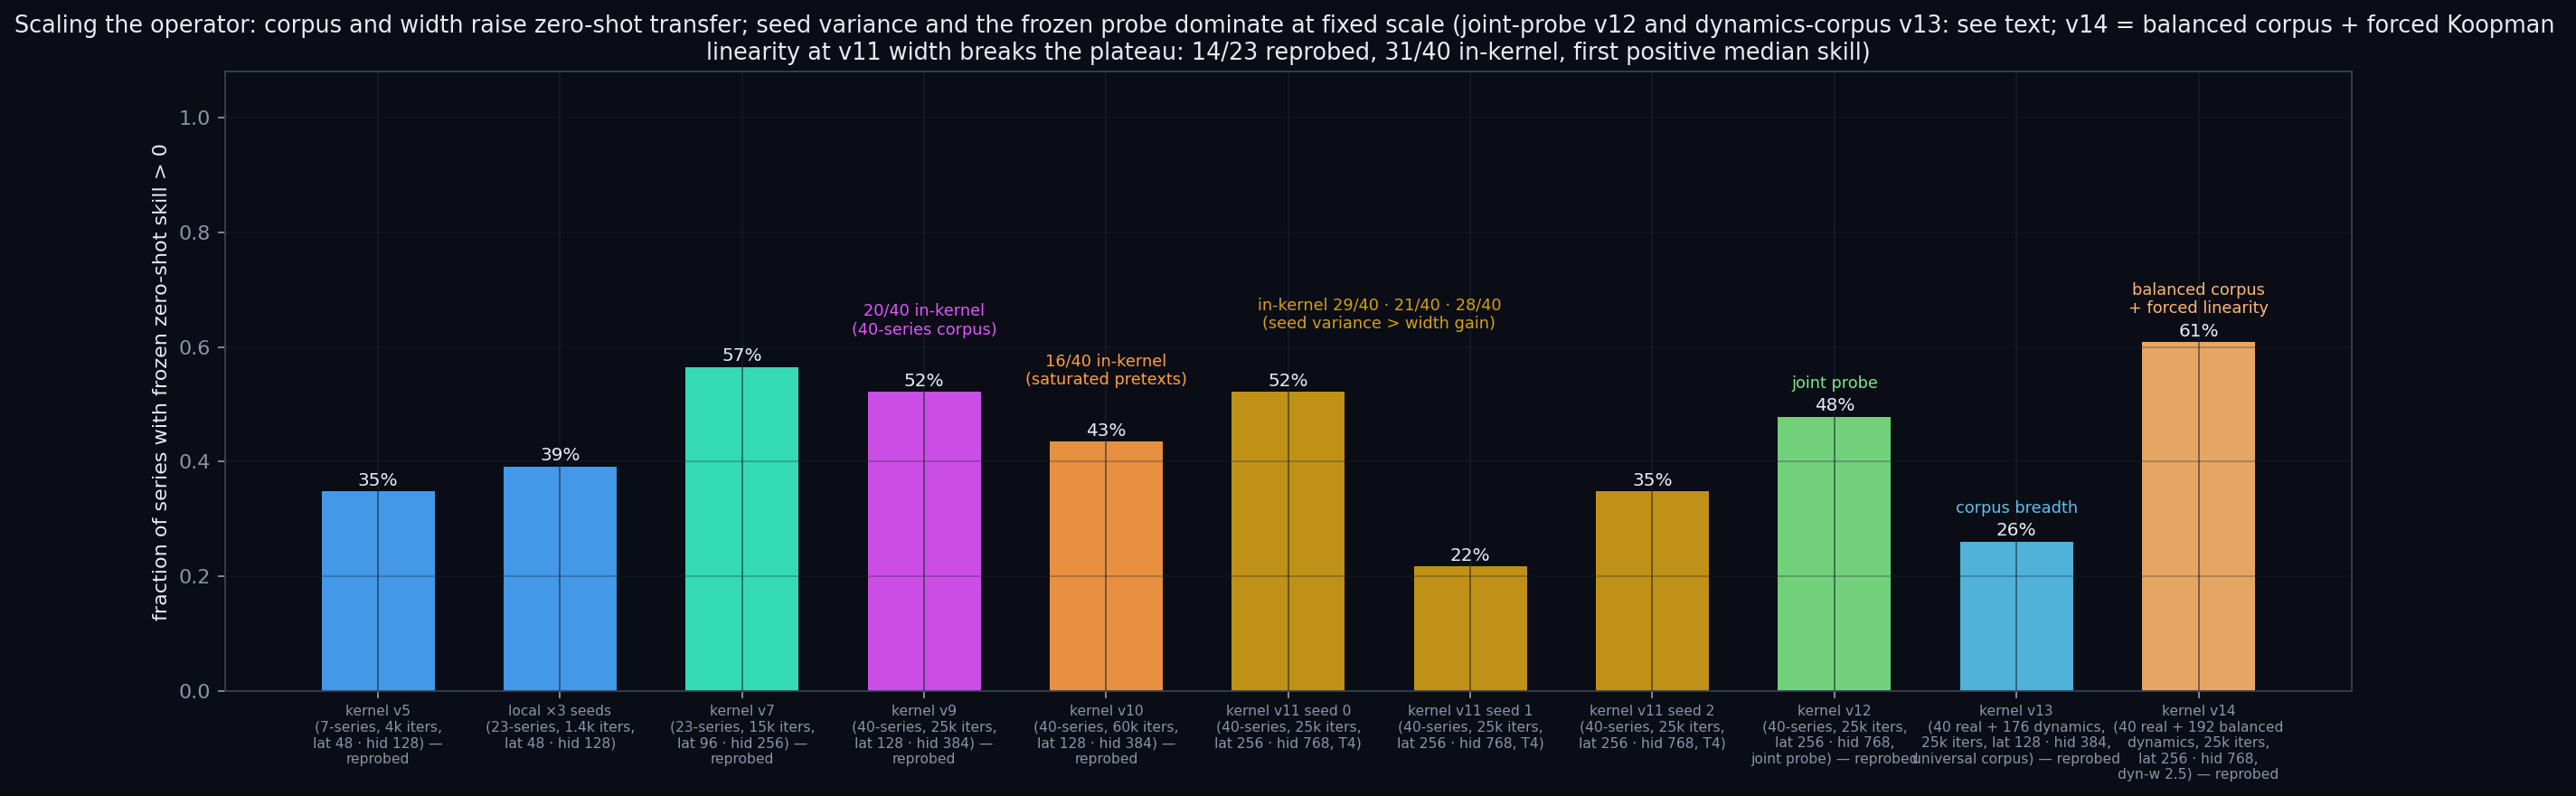
\includegraphics[width=0.85\textwidth]{fig_scaling.png}
\caption{Frozen-latent transfer across eleven training budgets on one shared
23-series corpus. Capacity, iterations and joint-probe regularization do not
move the plateau; the regime-balanced battery with forced Koopman linearity
does and replicates across seeds, while $25\times$ corpus breadth at fixed
budget regresses.}
\label{fig:scaling}
\end{figure}

\subsection{The matched-compute test: a negative result}
\label{sec:matched}
The corpus explanation is falsifiable: give the incumbent the operator's own
corpus at equal compute and the gap should shrink if it is purely a data effect.
We fine-tuned chronos-t5-small (46.2M parameters, pretrained on
$\sim$80{,}000 series) with the publisher's own tokenizer and objective on the
identical corpus used to pretrain the operator, and evaluated everything on the
identical 40 z-scored series, 0.7/0.2 split and skill-vs-persistence metric.

The prediction fails (Table~\ref{tab:matched}). At the parameter-matched budget
--- 1,127 steps, 52.0B parameter-steps, equal to the
operator's 2.08M $\times$ 25,000 = 52.0B --- fine-tuning
leaves Chronos statistically unchanged: median +22.70 against the true
frozen baseline's +21.42, 21W/19L,
$p$=0.98 (two-sided Wilcoxon). At 22$\times$ that
budget (1.15T parameter-steps) it improves only modestly and not
significantly (22W/18L, $p$=0.20; median
+33.34). Against the operator both checkpoints retain the frozen
model's advantage, at conventional significance (Chronos wins
24/40 against the frozen operator,
$p$=0.009; 27/40 at the matched budget,
$p$=0.012).

We report this as the paper's central negative result. It does \emph{not} show
that tokenization is superior --- the corpus is far too small to move a model
pretrained upstream on three orders of magnitude more data --- nor that
geometry is a dead end, since the operator's structural readouts have no
tokenizer analogue. It shows that at the compute scale we can afford,
\emph{pretraining scale dominates architecture}, and it delimits what a
geometry-first model must earn: a corpus of comparable breadth on which its
machinery faces an incumbent adapted to the same data. One methodological note
that strengthens the null: the kernel's in-run ``frozen'' column shared the
model object that fine-tuning mutated in place (correlation 0.986), so the
frozen baseline was re-measured post hoc on the byte-identical protocol.

\begin{table}[t]
\centering\small
\caption{Matched-compute test on the shared 40-series protocol. ``Frozen'' is
the untouched pretrained model re-measured on the identical protocol.}
\label{tab:matched}
\begin{tabular}{lccccc}
\toprule
model & params & param-steps & median skill & wins vs pers. & vs frozen \\
\midrule
TSO (frozen, ours) & 2.08M & 52.0B & +1.79 & 24/40 & --- \\
Chronos-t5-small frozen & 46.2M & --- & +21.42 & 28/40 & --- \\
\quad + matched fine-tune & 46.2M & 52.0B & +22.70 & 29/40 & 21W/19L \\
\quad + generous fine-tune & 46.2M & 1.15T & +33.34 & 31/40 & 22W/18L \\
\bottomrule
\end{tabular}
\end{table}

\subsection{What a frozen operator knows that a tokenizer does not}
\label{sec:geometry}
\textbf{The solar cycle, from a held-out channel.} The sunspot record is held
out of pretraining. At full rate it is amplitude-modulated noise and a one-step
linear fit of the frozen latent finds only trend. Coarsening it
$2\times,4\times,\dots,32\times$ --- the renormalization leg of the operator ---
collapses the fluctuation spectrum onto the cycle, which becomes a clean
eigenmode of the fitted Koopman matrix. The detected period is scale-covariant
and converges to the Schwabe cycle (128 months against
132 known, 3.0\% error; this record's FFT peak sits at
130.6 months). No regression is fitted on the cycle: it falls out of the
eigenvalues of a linear operator acting on a frozen cross-domain lift, stable
across hardware, width, corpus and objective (128--130 months for every
checkpoint we trained).

\textbf{Physics versus physiology, and tipping.} The same frozen latent, applied
to one synthetic chaotic channel and one real MIT-BIH record, keeps its top
Koopman eigenvalue pinned to the unit circle under $8\times$ decimation for
Lorenz-63 (0.999 $\to$ 0.937, scale-covariant physics) while a heartbeat sheds
spectral content (0.692 $\to$ 0.207, stochastic physiology): an unsupervised
physics-versus-physiology test from one model, full diagnostic in
Appendix~\ref{app:protocol}. Sweeping the Lorenz parameter $\rho$ from 1 to 40,
the Lyapunov estimator returns durably negative readings in the laminar regime
and a durable crossing to $\lambda_1>0$ at $\rho\approx21$ --- inside the
transient-chaos corridor that precedes the homoclinic explosion at
$\rho\approx24.74$ \cite{lorenz1963}. The raw series still looks unremarkable
while the geometry of the reconstructed attractor is already warping.

\textbf{Comparison with the incumbent, honestly framed.} Frozen
chronos-t5-small transfers better on median skill on the same protocol
(+21.42 against +1.79) and wins
24/40 head-to-head; that gap is the corpus (80{,}000
series against 40), and both foundation models beat the per-series token
baseline decisively (31/40 and 35/40). The operator is weakest on spiky,
near-unit-root series, where iterating a linear map for 100 steps amplifies any
latent error.

\begin{figure}[t]
\centering
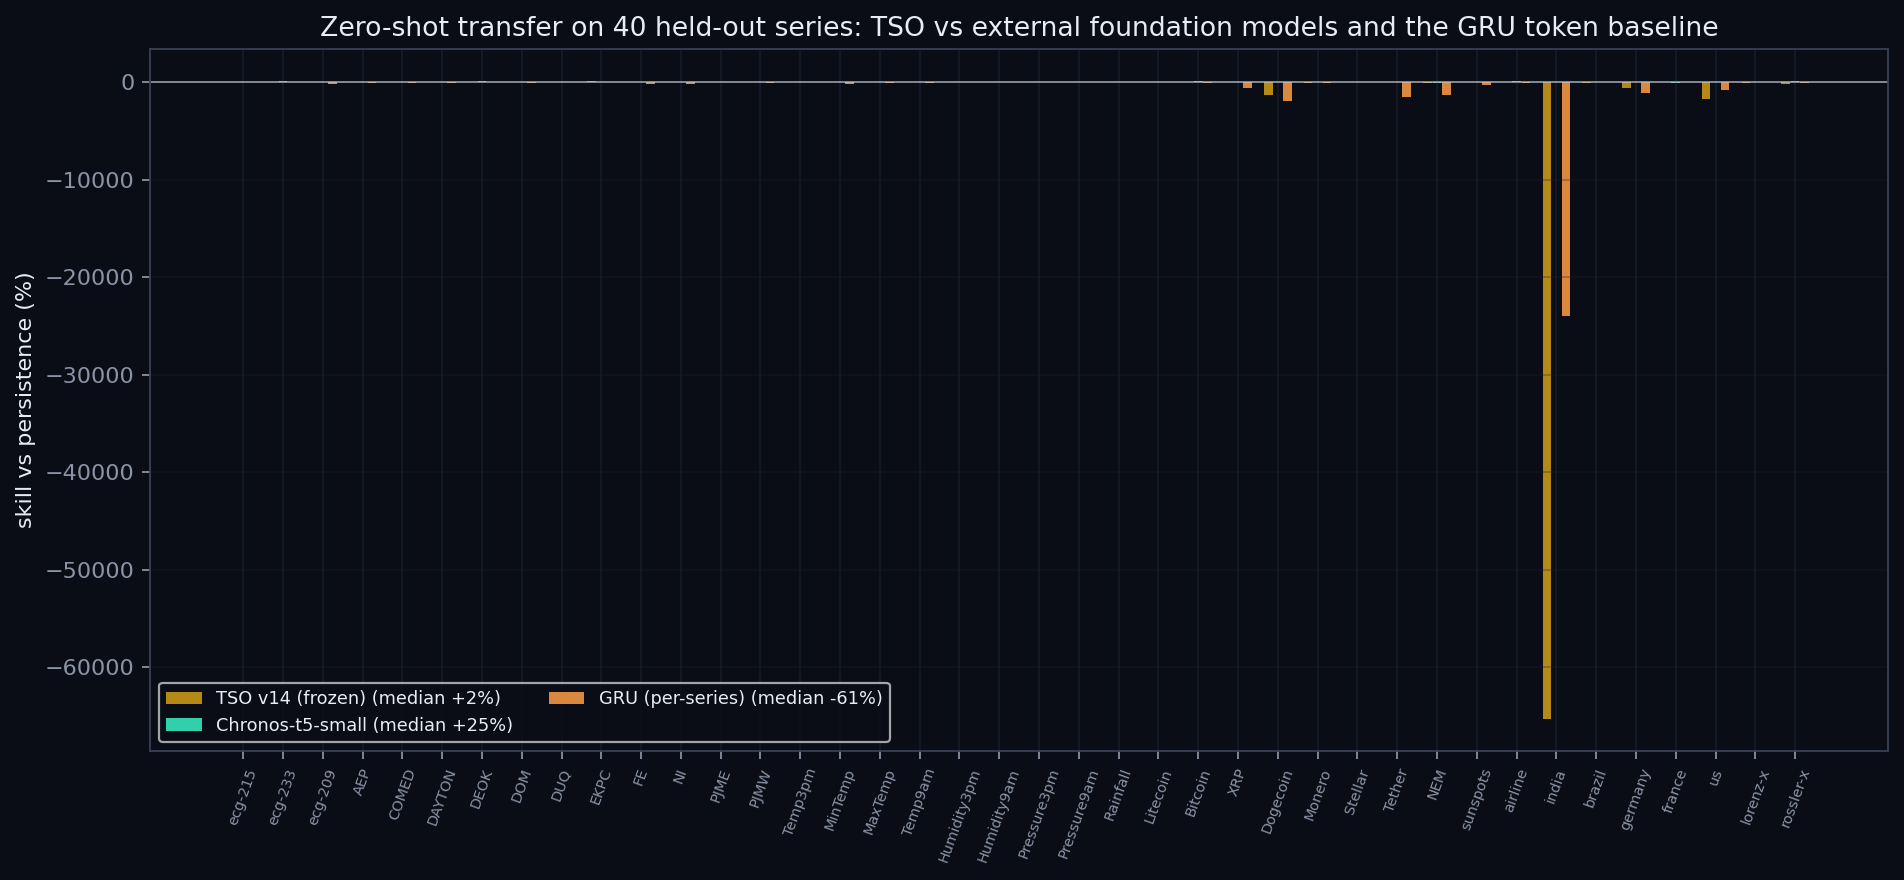
\includegraphics[width=0.43\textwidth]{fig_external.png}\hfill
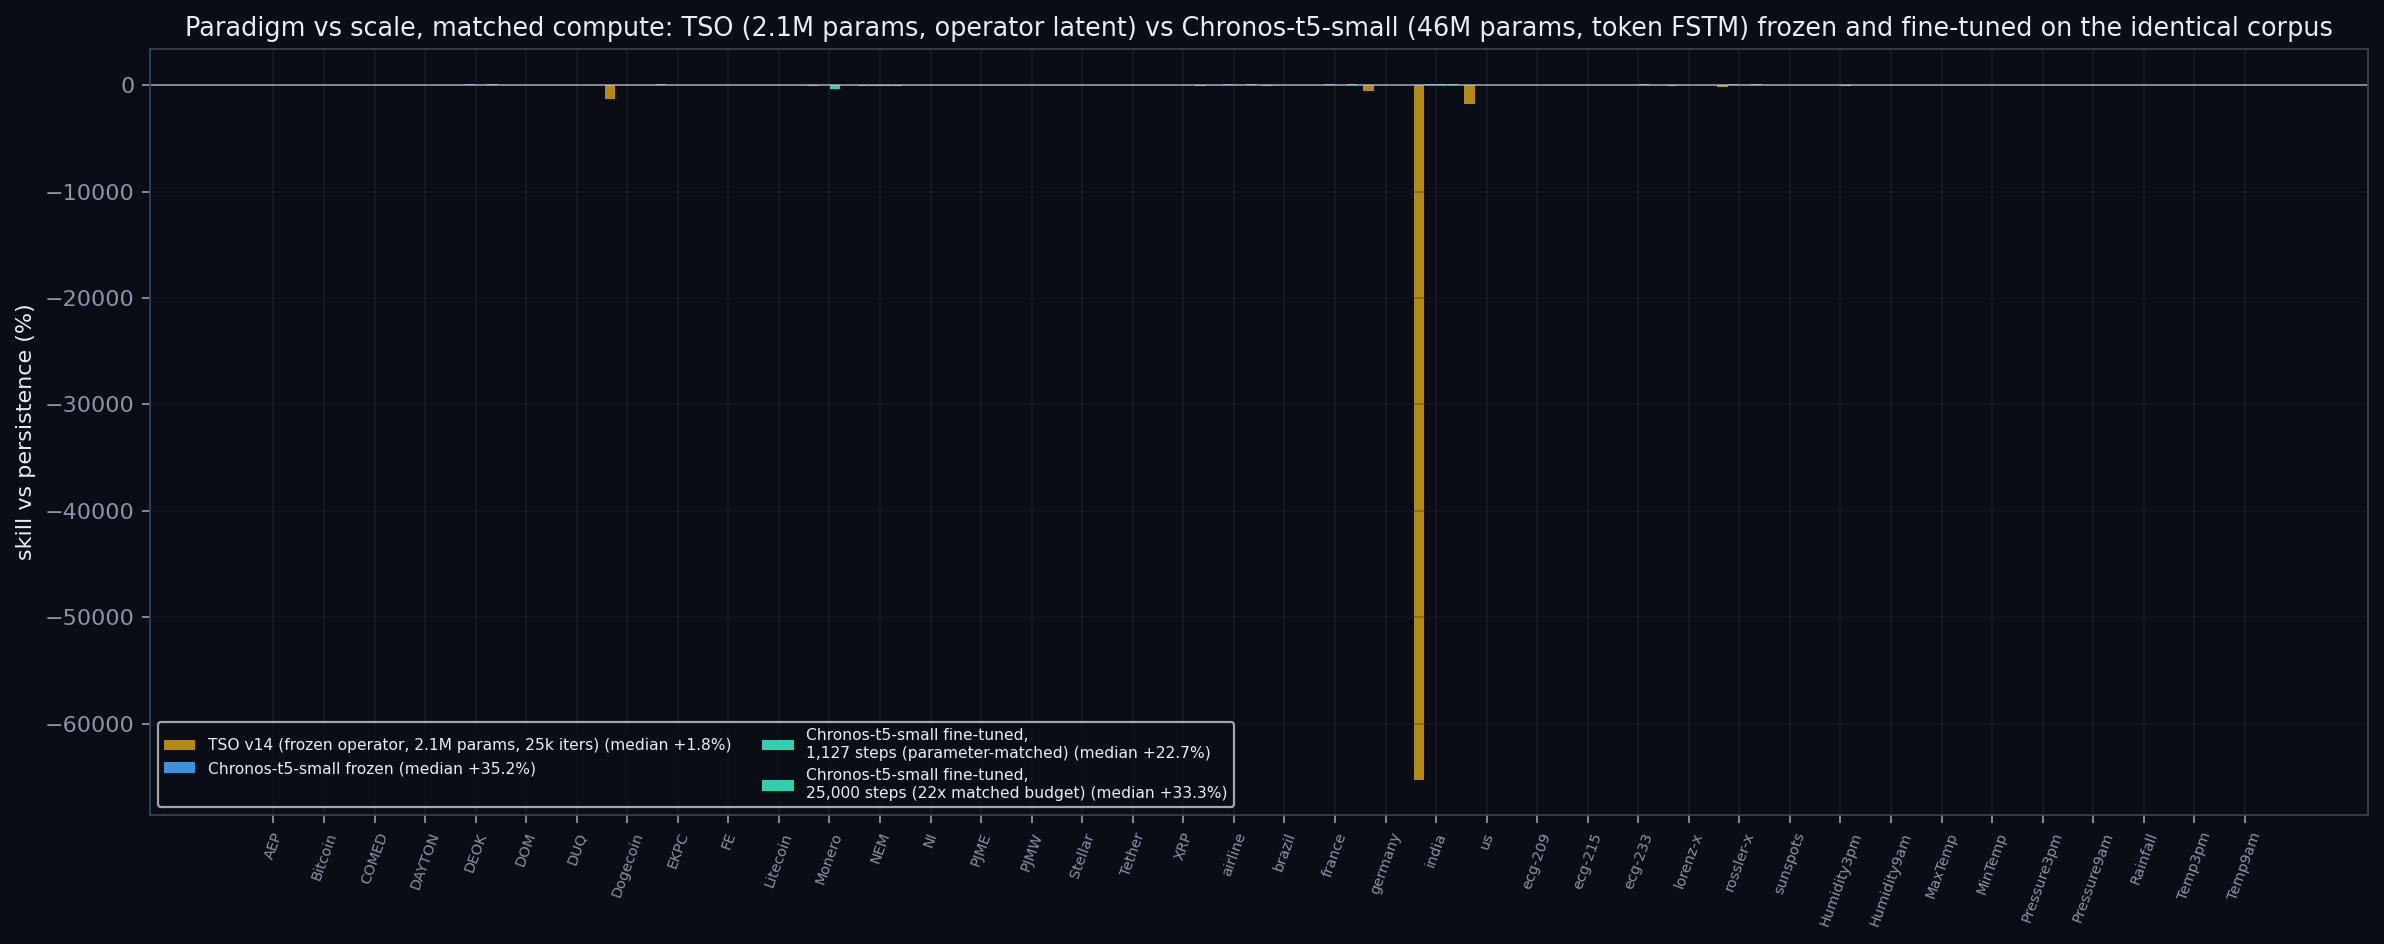
\includegraphics[width=0.43\textwidth]{fig_matched.png}
\caption{Left: zero-shot skill per series on the 40-series protocol, frozen
TSO against frozen Chronos and the GRU token baseline. Right: the
matched-compute test --- fine-tuning the incumbent on the operator's own corpus,
at equal parameter-steps and at 22$\times$ that budget, does not close the gap.}
\label{fig:external}
\end{figure}

\section{Discussion}
\label{sec:disc}
\textbf{Two axes of capability, not one.} A forecast-skill table measures one
axis. The operator's contributions lie on a second axis token models do not
produce: an unsupervised physics-versus-physiology diagnostic, a pre-onset
tipping detector, a spectral rediscovery of a physical constant, and a
phase-space object a human can inspect. Forecasting \emph{to} world modeling
should measure both, because a model can win the first while being blind to the
second, and vice versa.

\textbf{What has to be earned.} (i) \emph{Corpus}: 40 real series against the
incumbent's 80{,}000; since breadth at fixed compute trades against per-series
exposure, the next step is more series \emph{and} proportionally more compute.
(ii) \emph{A differentiable probe}: the plateau sits at the frozen closed-form
evaluation interface, since regularizing latent linearizability during
pretraining does not move it. (iii) \emph{Probabilistic roll-outs}: a
deterministic linear map explodes on near-unit-root and spiky series. (iv)
\emph{Irregular sampling}: connecting the continuous-time delay-embedding view
to state-space and neural-operator architectures is the route to genuinely
asynchronous multi-rate data.

\textbf{Limitations and conclusion.} The corpus is small (40 real series, 8
domains, up to 36k samples), surviving effects are directional rather than
asymptotic, and the matched-compute experiment cannot separate ``tokenization
is the wrong prior'' from ``46M parameters on 40 series is too little''.
Free-tier hardware is a reproducibility virtue and also the reason the operator
was never trained at foundation scale. Still, a foundation model of temporal
systems should hold the geometry of a system, not only its next value: we built
one, measured it against an incumbent, and found that the same latent delivers
structural knowledge no tokenizer produces. The remaining gap is measured, not
mysterious.

\begin{thebibliography}{9}
\bibitem{chronos2024} A.~F.~Ansari et al. Chronos: learning the language of
time series. \emph{TMLR} (2024). arXiv:2403.07815.
\bibitem{timesfm2024} A.~Das, W.~Kong, R.~Sen, Y.~Zhou. A decoder-only
foundation model for time-series forecasting. \emph{ICML} (2024).
\bibitem{moirai2024} G.~Woo et al. Unified training of universal time series
forecasting transformers. \emph{ICML} (2024).
\bibitem{takens1981} F.~Takens. Detecting strange attractors in turbulence.
\emph{Lecture Notes in Mathematics} 898, 366--381 (1981).
\bibitem{kennel1992} M.~B.~Kennel, R.~Brown, H.~D.~I.~Abarbanel. Determining
embedding dimension for phase-space reconstruction using a geometrical
construction. \emph{Phys.\ Rev.\ A} 45, 3403 (1992).
\bibitem{koopman1931} B.~O.~Koopman. Hamiltonian systems and transformation in
Hilbert space. \emph{PNAS} 17, 315--318 (1931).
\bibitem{mezic2005} I.~Mezi\'c. Spectral properties of dynamical systems,
model reduction and decompositions. \emph{Nonlinear Dyn.} 41, 309--325 (2005).
\bibitem{schmid2010} P.~J.~Schmid. Dynamic mode decomposition of numerical and
experimental data. \emph{J.\ Fluid Mech.} 656, 5--28 (2010).
\bibitem{williams2015} M.~O.~Williams, I.~G.~Kevrekidis, C.~W.~Rowley. A
data-driven approximation of the Koopman operator: extending dynamic mode
decomposition. \emph{J.\ Nonlinear Sci.} 25, 1307--1346 (2015).
\bibitem{lusch2018} B.~Lusch, S.~L.~Kutz, J.~N.~Brunton. Deep learning for
universal linear embeddings of nonlinear dynamics. \emph{Nature Commun.} 9,
4950 (2018).
\bibitem{wolf1985} A.~Wolf, J.~B.~Swift, H.~L.~Swinney, J.~A.~Vastano.
Determining Lyapunov exponents from a time series. \emph{Physica D} 16,
285--317 (1985).
\bibitem{lorenz1963} E.~N.~Lorenz. Deterministic nonperiodic flow.
\emph{J.\ Atmos.\ Sci.} 20, 130--141 (1963).
\bibitem{li2021fno} Z.~Li et al. Fourier neural operator for parametric partial
differential equations. \emph{ICLR} (2021).
\bibitem{chen2018node} R.~T.~Q.~Chen, Y.~Rubanova, J.~Bettencourt, D.~Duvenaud.
Neural ordinary differential equations. \emph{NeurIPS} (2018).
\bibitem{gu2023mamba} A.~Gu, T.~Dao. Mamba: linear-time sequence modeling with
selective state spaces. \emph{COLM} (2024).
\bibitem{kaplan2020} J.~Kaplan et al. Scaling laws for neural language models.
\emph{arXiv:2001.08361} (2020).
\end{thebibliography}

\newpage
\appendix
\section{Core pipeline and in-kernel comparison}
\label{app:tables}
Table~\ref{tab:core} gives the full scale-space diagnostic summarised in
Section~\ref{sec:geometry}, and Table~\ref{tab:kernel} the per-run 40-series
comparison against the GRU token baseline summarised in
Section~\ref{sec:transfer}; Fig.~\ref{fig:solar} shows the scale-covariant solar
readout and the reconstructed Lorenz attractor. Every number here is produced
by the same scripts as the body text.

\begin{figure}[h]
\centering
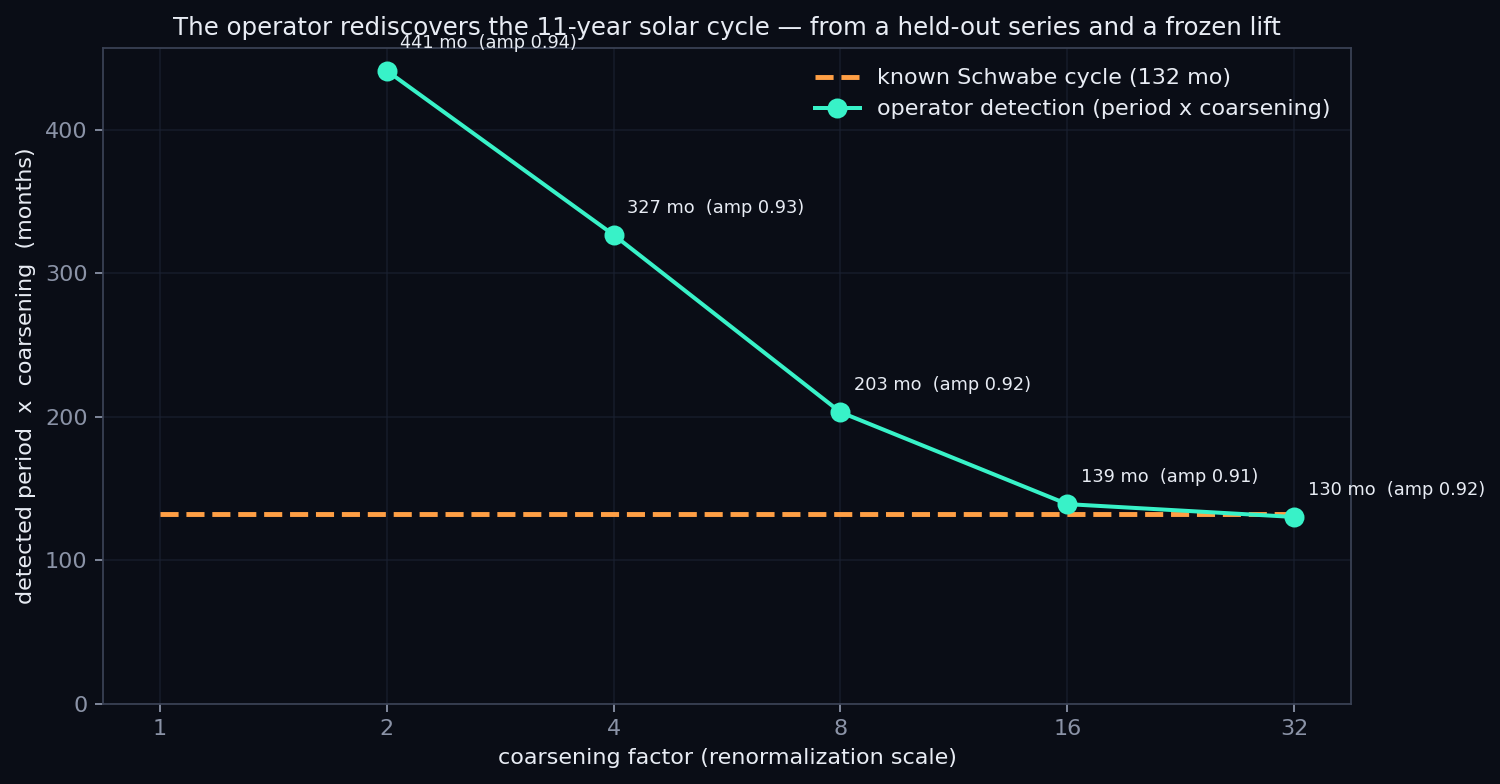
\includegraphics[width=0.52\textwidth]{fig_solar_discovery.png}\hfill
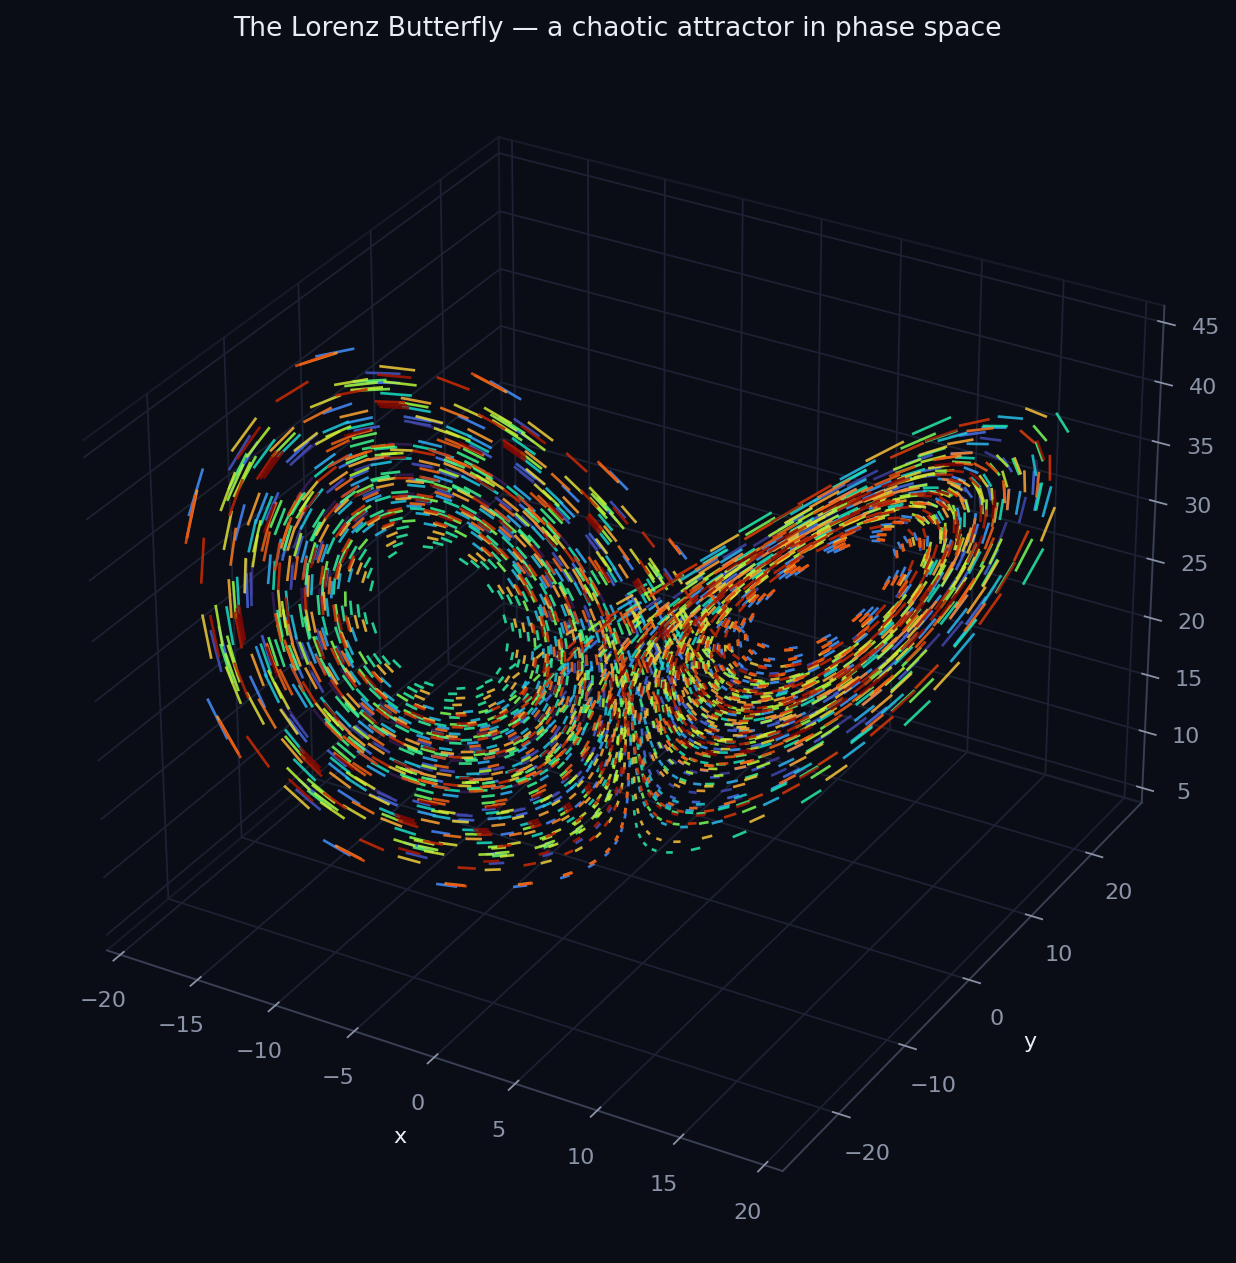
\includegraphics[width=0.26\textwidth]{attractor_butterfly.png}
\caption{Left: the scale-covariant period readout on the held-out sunspot
record converging to the 11-year Schwabe cycle. Right: the reconstructed Lorenz
attractor as the operator sees it --- a phase-space object, not a token stream.}
\label{fig:solar}
\end{figure}

\begin{table}[h]
\centering\small
\caption{Core operator on one synthetic chaotic system and one real
physiological record. Skill is \% RMSE reduction over persistence on the
held-out horizon; $|\lambda|$ is the top Koopman eigenvalue magnitude under
$1\times$ and $8\times$ block decimation.}
\label{tab:core}
\begin{tabular}{lcc}
\toprule
 & Lorenz-63 $x$ (chaos) & MIT-BIH RR (heartbeats) \\
\midrule
delay $\tau$ / embedding dimension $m$ & 59 / 3 & 1 / 6 \\
samples & 4{,}000 (RK4) & 2,500 \\
eDMD-RFF skill (\%) & +21.3 & +3.3 \\
plain DMD skill (\%) & +18.2 & +3.3 \\
top $|\lambda|$, $1\times$ $\to$ $8\times$ & 0.999 $\to$ 0.937 & 0.692 $\to$ 0.207 \\
neural vector field, short-horizon corr. & 0.79 & 0.74 \\
neural field loss & 0.022 & 0.152 \\
\bottomrule
\end{tabular}
\end{table}

\begin{table}[h]
\centering\small
\caption{In-kernel 40-series comparison against the per-series GRU token
baseline (identical hardware, split and metric). Median advantage is over
persistence. Dashes: value not recorded for that run.}
\label{tab:kernel}
\begin{tabular}{lccc}
\toprule
run & TSO wins vs GRU & $p$ & median skill (pts) \\
\midrule
v9 & 28/40 & $p$=0.017 & +46.5 \\
v11 & 29/40 & $p$=0.002 & +60.9 \\
v12 & 28/40 & --- & +59.2 \\
v13 & 25/40 & --- & +58.0 \\
v14 & 31/40 & $p$<0.001 & +57.2 \\
\bottomrule
\end{tabular}
\end{table}

\section{Protocol, provenance and per-series detail}
\label{app:protocol}
\textbf{Hardware and framework.} All corpora were fetched through the Kaggle
legacy API into Kaggle kernels (CPU and NVIDIA GPU sessions, mixed precision
when CUDA was available) and analysed locally; every script in this paper is
runnable end to end from the corpora alone.

\textbf{Evaluation protocol.} Series are z-scored, split 0.7/0.2, embedded with
per-series $\tau$, probed closed-form, and scored by RMSE reduction against
persistence over horizon $\min(20\%\,n,100)$. Paired comparisons use the
two-sided binomial sign test on win counts (magnitudes are skewed by a few
explosive series, so medians and Wilcoxon signed-rank tests are reported
alongside means). The matched-compute budget is defined in parameter-steps,
not wall-clock: the operator's 2.08M parameters $\times$ 25{,}000 iterations
equals chronos-t5-small's 46.2M parameters $\times$ 1{,}127 steps.

\textbf{Corpora.} Eight domains: grid electricity demand (10 regions),
weather (4 channels), cryptocurrency (3), COVID-19 daily cases (5 countries,
held out), MIT-BIH cardiac records (2, held out), air-passenger counts,
sunspots (held out) and synthetic physics. Public dataset slugs used:
\texttt{robikscube/hourly-energy-consumption},
\texttt{jsphyg/weather-dataset-rattle-package},
\texttt{sudalairajkumar/cryptocurrencypricehistory},
\texttt{imdevskp/corona-virus-report},
\texttt{sumit042004/cardiac-arrhythmia-ecg-dataset-mit-bih},
\texttt{rakannimer/air-passengers}, \texttt{robervalt/sunspots}.

\textbf{What is not claimed.} We do not claim state-of-the-art forecasting.
We do not claim that tokenization is wrong. We do not claim that the operator
scales --- we claim that the experiment that would decide that has been
specified, run at the largest scale available to us, and reported in full.

\section{Use of AI assistants}
\label{app:ai}
Following the workshop's policy on LLM and agent use: an AI coding assistant
was used for implementation, experiment orchestration (writing, launching and
polling the compute kernels), figure generation and LaTeX drafting under
direct author supervision. All experimental design decisions, the choice of
baselines and metrics, the interpretation of results, and every number and
claim in this paper were reviewed and verified against the stored artefacts
(JSON metric files, kernel logs and per-series evaluations) by the author,
who takes full responsibility for the content.

\section{Reproduction commands}
\label{app:repro}
\textbf{Core pipeline and scale-space diagnostic:}
\texttt{python scripts/study\_experiments.py}.
\textbf{Foundation pretraining (local, 3 seeds):}
\texttt{python scripts/pretrain\_foundation.py}.
\textbf{Kernel build + launch (all scaling and matched-compute runs):}
\texttt{python scripts/build\_kernel\_single.py}; the kernel is a single
self-contained script that mounts the datasets, pretrains, evaluates every
baseline on identical hardware and writes metrics, figures and checkpoints.
\textbf{Matched-compute analysis:}
\texttt{python scripts/v18\_final\_analysis.py}.
\textbf{This paper:} \texttt{python scripts/study\_paper\_neurips.py}.

\end{document}
